% !TeX root = ../bbchallenge-paper.tex

\newpage
\subsection{Weighted FAR (WFAR)}\label{sec:WFAR}

% 1RB---_0RC1LC_1RD1RC_1LE1LD_0RA0LE
% 1RB---_0RC1LB_1RD1RC_1LE1LD_0RA0LE
% 1RB---_0RC1RC_1RD1RC_1LE1LD_0RA0LE
% 1RB---_0RC1RC_1RD1RB_1LE1LD_0RA0LE *
% 1RB1RA_1LC1LB_0RD0LC_1RE---_0RA1RA
% 1RB1RA_1LC1LB_0RD0LC_1RE---_0RA1LA
% 1RB1RA_1LC1LB_0RD0LC_1RE---_0RA1LE
% 1RB1RE_1LC1LB_0RD0LC_1RE---_0RA1RA
% 1RB1RA_1LC1LE_0RD0LC_1RE---_0RA1LB
% 1RB---_0RC1LD_1RD1RC_1LE1LB_0RA0LE
% 1RB1RE_1LC1LB_0RD0LC_1LE---_0RA1RA
% 1RB---_0LC1LC_1LD1LB_1RE1RD_0LA0RE
% 1RB1LC_1LC1RA_0LE0LD_0RA1RD_---0LC *
% 1RB1LC_1LB1RA_0LE0LD_0RA1RD_---0LC
% 1RB0RC_1LC0LE_0LD0LB_1RA---_1LB0RD
% 1RB0RE_0RC0RA_1LD---_1LA0LB_1RA0LC
% 1RB0LD_1RC0RA_0RD0RB_1LE---_1LB0LC *
\usetikzlibrary{automata, positioning, arrows.meta}
\begin{figure}[h]
    \centering
    \begin{minipage}[t]{0.23\textwidth}
        \raggedright
        (a) Turing machine \\
        \centering
        \vspace{0.6em}
        \begin{tabular}{ccc}
            \toprule
                    & \textbf{0} & \textbf{1} \\
            \midrule
            \stateA & 1R\stateB  & ---        \\
            \stateB & 0R\stateC  & 1L\stateC  \\
            \stateC & 1R\stateD  & 1R\stateC  \\
            \stateD & 1L\stateE  & 1L\stateD  \\
            \stateE & 0R\stateA  & 0L\stateE  \\
            \bottomrule
        \end{tabular}

        \vspace{1em}
        \raggedright
        (a') Space-time diagram \\
        \vspace{0.3em}
        \centering
        \includegraphics[width=1.1\linewidth]{figures/space-time-diagrams/counter_wfar.png}
    \end{minipage}
    \hfill
    \vrule
    \hfill
    \begin{minipage}[t]{0.71\textwidth}

        \begin{minipage}[t]{1\linewidth}

            \begin{minipage}[t]{0.49\textwidth}
                \raggedright
                (b) Left Weighted Automaton \\
                \vspace{0.5em}
                \centering
                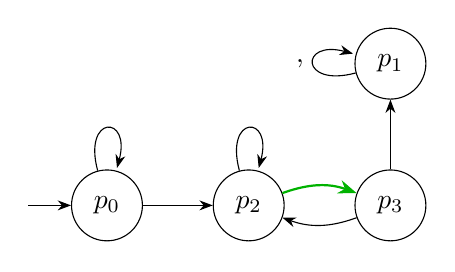
\begin{tikzpicture}[->, >=Stealth, auto, node distance=1.8cm, every node/.style={scale=1}]
                    \tikzset{
                        state/.style={
                                circle, draw, minimum size=0.9cm, inner sep=1pt
                            }
                    }

                    % States
                    \node[state] (0) {$p_0$};
                    \node[state] (2) [right of=0] {$p_2$};
                    \node[state] (3) [right of=2] {$p_3$};
                    \node[state] (1) [above of=3] {$p_1$};

                    % Initial arrow
                    \draw[->] (-1,0) -- (0);

                    % Transitions
                    \draw[->, black] (0) edge[loop above] node{\szero} (0);
                    \draw[->, black] (0) edge node{\sone} (2);

                    \draw[->, black] (2) edge[loop above] node{\sone} (2);
                    \draw[->, black, bend left=20] (3) to node{\sone} (2);
                    \draw[->, green!70!black, thick, bend left=20] (2) to node{\szero} (3);

                    \draw[->, black] (3) edge node{\szero} (1);
                    \draw[->, black] (1) edge[loop left] node{\szero, \sone} (1);


                \end{tikzpicture}
            \end{minipage}
            \hfill
            \begin{minipage}[t]{0.49\textwidth}
                \raggedright
                (c) Right Weighted Automaton \\
                \vspace{0.3em}
                \centering
                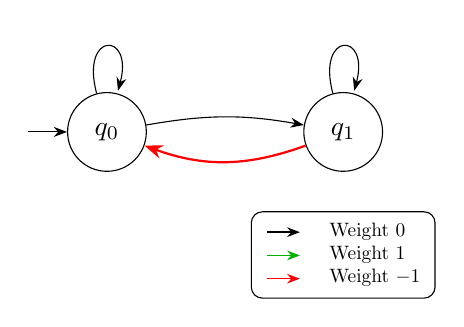
\begin{tikzpicture}[->, >=Stealth, auto, node distance=2cm, every node/.style={scale=1}]
                    \tikzset{
                        state/.style={
                                circle, draw, minimum size=1cm, inner sep=1pt
                            }
                    }

                    % % Upper isolated state
                    % \node[state] (1top) at (0,2.5) {1};
                    % \draw[->] (1top) edge[loop above] node{1} (1top);
                    % \draw[->] (1top) edge[loop left] node{0} (1top);

                    % Lower automaton
                    \node[state] (0) at (0,0) {$q_0$};
                    \node[state] (2) at (3,0) {
                        $q_1$};

                    \draw[->] (0) edge[loop above] node{\szero} (0);
                    \draw[->] (2) edge[loop above] node{\sone} (2);

                    \draw[->] (0) edge[bend left=10] node{\sone} (2);
                    \draw[->, red, bend left=20, thick] (2) to node[below]{\szero} (0);

                    % Initial state arrow
                    \draw[->] (-1,0) -- (0);

                    % Compact and aligned legend
                    \node[draw, below=0.5cm of 2, inner sep=3pt, rounded corners] (legend) {
                        \scalebox{0.7}{
                            \begin{tabular}{@{}rl@{}}
                                \tikz[baseline=-0.5ex]\draw[->, black, thick] (0,0) -- +(0.6,0);          & \;Weight 0    \\
                                \tikz[baseline=-0.5ex]\draw[->, green!70!black, thick] (0,0) -- +(0.6,0); & \;Weight 1    \\
                                \tikz[baseline=-0.5ex]\draw[->, red, thick] (0,0) -- +(0.6,0);            & \;Weight $-1$
                            \end{tabular}
                        }
                    };
                \end{tikzpicture}
            \end{minipage}

            % \vspace{1em}
            % $\rightarrow$ \quad 1\,0\,|\,0\,|\,0\,1 \\
            % \vspace{0.5em}
            % $+\;4$

        \end{minipage}

        \vspace{1em}

        \raggedright
        (d) Example: configuration is accepted, hence nonhalting \\
        \vspace{0.3em}
        \centering

        \newcommand{\underarrowleft}[1]{%
            \tikz[baseline=(X.base)]{
                \node (X) {$#1$};
                \draw[->, thick] ([yshift=-1.3ex]X.east) -- ([yshift=-1.3ex]X.west);
            }
        }

        \newcommand{\underarrowright}[1]{%
            \tikz[baseline=(X.base)]{
                \node (X) {$#1$};
                \draw[->, thick] ([yshift=-1.3ex]X.west) -- ([yshift=-1.3ex]X.east);
            }
        }

        \scalebox{0.8}{

            \begin{minipage}{\textwidth}
                \centering
                {\LARGE
                $\underarrowright{\texttt{10101}}\; \texttt{\stateC}\sone\; \underarrowleft{\texttt{01}}$ \\
                \vspace{-0.3em}
                {\small $\quad\quad$Left WA reads$\quad\quad\quad\quad\quad\quad\quad\quad$Right WA reads} \\
                %\vspace{0.1em}
                $\quad  \; \;$\fcolorbox{red}{yellow!30}{$[p_2] \; \texttt{\stateC}\sone\; [q_0]$} \\
                \vspace{-2em}
                \[
                    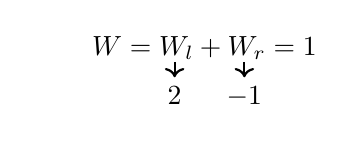
\begin{tikzpicture}[baseline=(base)]
                        \node (base) {$\quad \quad W = W_l + W_r = 1$};

                        \coordinate (Wl) at ([xshift=5.33em]base.base west);
                        \coordinate (Wr) at ([xshift=7.85em]base.base west);

                        % Labels
                        \node[below=1.8ex of Wl] (lval) {\normalsize 2};
                        \node[below=1.8ex of Wr] (rval) {\normalsize $-1$};

                        % Arrows pointing down from W_l and W_r
                        \draw[->, thick] ([yshift=-0.5ex]Wl) -- (lval.north);
                        \draw[->, thick] ([yshift=-0.5ex]Wr) -- (rval.north);
                    \end{tikzpicture}
                \] \\
                \vspace{-0.5em}
                {\large Configuration accepted, see (e) }
                }
                % \begin{tikzpicture}[->, >=Stealth, auto, node distance=2cm, every node/.style={scale=1}]
                %     \tikzset{
                %         state/.style={
                %                 circle, draw, minimum size=1cm, inner sep=1pt
                %             }
                %     }

                %     % % Upper isolated state
                %     % \node[state] (1top) at (0,2.5) {1};
                %     % \draw[->] (1top) edge[loop above] node{1} (1top);
                %     % \draw[->] (1top) edge[loop left] node{0} (1top);

                %     % Lower automaton
                %     \node[state] (0) at (0,0) {0};
                %     \node[state] (2) at (3,0) {1};

                %     \draw[->] (0) edge[loop above] node{0} (0);
                %     \draw[->] (2) edge[loop above] node{1} (2);

                %     \draw[->] (0) edge[bend left=10] node{1} (2);
                %     \draw[->, red, bend left=20, thick] (2) to node[below]{0} (0);

                %     % Initial state arrow
                %     \draw[->] (-1,0) -- (0);
                % \end{tikzpicture}
            \end{minipage}
        }

        \vspace{0.5em}
        \raggedright
        (e) Accepted weighted configurations \\
        \centering

        \usetikzlibrary{positioning, shapes.multipart, fit}
        \begin{tikzpicture}[node distance=0.2cm and 0.3cm, every node/.style={font=\footnotesize}, anchor=north]

            % Reference coordinate for top alignment
            \coordinate (topref) at (0,0);

            % W >= -1 group
            \node[draw, rectangle, rounded corners, inner sep=3pt] (wmin1box)
            {\begin{tabular}{l}
                    $[p_2]\; \texttt{\stateE}\szero\; [q_0]$
                \end{tabular}};
            \node[above=0cm of wmin1box] {$W \geq$ -1};

            % W = 0 group
            \node[draw, rectangle, rounded corners, inner sep=3pt, right=of wmin1box] (w0box)
            {\begin{tabular}{l}
                    $[p_0]\; \texttt{\stateA}\szero\; [q_0]$ \\
                    $[p_0]\; \texttt{\stateE}\szero\; [q_0]$ \\
                    $[p_0]\; \texttt{\stateE}\sone\; [q_0]$
                \end{tabular}};
            \node[above=0cm of w0box] {$W = 0$};

            % W >= 0 group
            \node[draw, rectangle, rounded corners, inner sep=3pt, right=of w0box] (w0plusbox)
            {\begin{tabular}{l}
                    $[p_2]\; \texttt{\stateB}\szero\; [q_0]$ \\
                    $[p_2]\; \texttt{\stateE}\sone\; [q_0]$  \\
                    $[p_3]\; \texttt{\stateE}\sone\; [q_0]$
                \end{tabular}};
            \node[above=0cm of w0plusbox] {$W\geq0$};
            % W >= 1 group
            \node[draw, rectangle, rounded corners, inner sep=3pt, below=0.6cm of w0box, xshift=1.4cm] (w1box)
            {\begin{tabular}{ll}
                    $[p_3]\; \texttt{\stateA}\szero\; [q_1]$                                             & $[p_2]\; \texttt{\stateC}\sone\; [q_1]$  \\
                    $[p_2]\; \texttt{\stateB}\szero\; [q_1]$                                             & $[p_3]\; \texttt{\stateC}\sone\; [q_1]$  \\
                    $[p_2]\; \texttt{\stateB}\sone\; [q_0]$                                              & $[p_2]\; \texttt{\stateD}\szero\; [q_0]$ \\
                    $[p_2]\; \texttt{\stateB}\sone\; [q_1]$                                              & $[p_2]\; \texttt{\stateD}\szero\; [q_1]$ \\
                    $[p_2]\; \texttt{\stateC}\szero\; [q_0]$                                             & $[p_2]\; \texttt{\stateE}\sone\; [q_1]$  \\
                    $[p_3]\; \texttt{\stateC}\szero\; [q_0]$                                             & $[p_3]\; \texttt{\stateE}\sone\; [q_1]$  \\
                    \rule{0pt}{3.3ex}\fcolorbox{red}{yellow!30}{$[p_2]\; \texttt{\stateC}\sone\; [q_0]$} &                                          \\
                \end{tabular}};
            \node[above=0cm of w1box] {$W \geq 1$};

            % W >= 2 group
            \node[draw, rectangle, rounded corners, inner sep=6pt, below=0.7cm of wmin1box] (w2box)
            {\begin{tabular}{l}
                    $[q_3]\; \texttt{\stateA}\szero\; [q_0]$ \\
                    $[q_2]\; \texttt{\stateC}\szero\; [q_1]$ \\
                    $[q_3]\; \texttt{\stateC}\szero\; [q_1]$ \\
                    $[q_3]\; \texttt{\stateC}\sone\; [q_0]$  \\
                    $[q_2]\; \texttt{\stateD}\sone\; [q_0]$  \\
                    $[q_2]\; \texttt{\stateD}\sone\; [q_1]$  \\
                    $[q_3]\; \texttt{\stateD}\sone\; [q_1]$  \\
                \end{tabular}};
            \node[above=0cm of w2box] {$W \geq 2$};

        \end{tikzpicture}

    \end{minipage}

    \caption{TODO}
\end{figure}

% \vspace{5em}
% \raggedright
% (e) Accepted weighted configurations \\
% \vspace{-1em}
% \footnotesize
% \begin{minipage}[t]{0.48\textwidth}
%     \begin{align*}
%          & [3]\; \text{\stateA}0\; [0];\; W \geq 0 \\
%          

%          & [2]\; \text{\stateC}0\; [1] \\

%          & [3]\; \text{\stateC}0\; [1] \\

%          & [3]\; \text{\stateC}1\; [0] \\

%     \end{align*}
% \end{minipage}
% \hfill
% \vrule width 0.5pt
% \hfill
% \begin{minipage}[t]{0.48\textwidth}
%     \begin{align*}

%          & \;[2]\; \text{\stateD}1\; [0] \\
%          & \;[2]\; \text{\stateD}1\; [1] \\
%          & \;[3]\; \text{\stateD}1\; [1] \\

%     \end{align*}